\documentclass[FinalReport.tex]{subfiles}
\begin{document}

\bigskip

\section*{\textsc{\Large Discussion}}
 Examining the execution times of each configuration for the separate traces is not a useful way to measure configuration performance.  The execution time is dependent on the number of instructions in each trace file, and so varies both by configuration and trace size.  To eliminate this variable, we divided the execution time or cycles by the number of references in each trace to find the CPI.  This can seen in Fig.~\ref{fig:CPI}.
 
	The most noteworthy feature of Fig.~\ref{fig:CPI} is the variable dependence of trace files on configuration.  Both traces libquantum and bzip demonstrate extremely low variance across configurations, while traces such as onmetpp and sjeng demonstrate high variance. This variance is due to function and structure of the code written for these trace files. For example, it is likely that libquantum and bzip frequently reference spatial dissimilar locations in memory, making the spatial locality benefit of caching obsolete. Additionally, if libquantum and bzip were written sequentially and do not frequently loop, the benefit of temporal locality in caching is lost. Traces onmetpp and sjeng however are examples of code that frequently references spatially and temporally similar locations of memory. Frequent looping and indexing of large, static data arrays are good examples of this.
	
	 When considering the best performing configuration, it is useful to consider the average instructions per cycle versus configuration. Fig.~\ref{fig:IPC} demonstrates this relationship. An optimally designed multi-purpose architecture should maximize the IPC for all traces. The fully associative cases exhibit the highest instructions per cycle for all traces. This is because a fully associative cache utilizes a least recently used (LRU) buffer for a single set. In direct mapped and non-fully associative configurations multiple locations in memory or lower tier caches can reference the same index and cause the cache to miss.  In the fully associative case, the LRU determines what block is overwritten based on temporal locality.  

\begin{figure}[H]
\centering
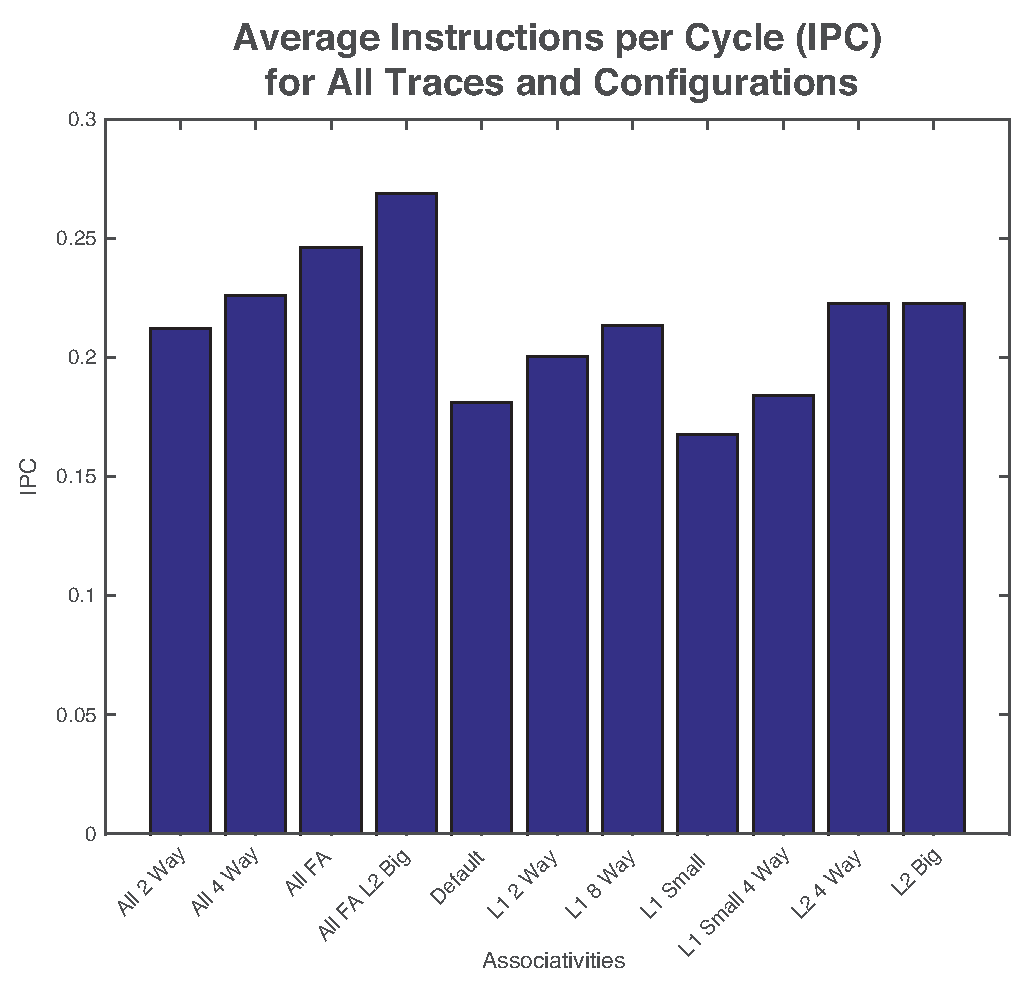
\includegraphics[scale = 0.75]{IPC.eps}
\caption{Average IPC for each configuration\label{fig:IPC}}
\end{figure}

Pure instructions per cycle performance however is not the only consideration to make when choosing the best machine. Cost is an important factor. While the FA configurations are the fastest on average, they are also the most expensive. FA caches are extremely expensive, and in the simulation according to specifications cost in the thousands of dollars. When considering what system to buy, it is therefore useful to look at IPC per dollar, as seen in Fig.~\ref{fig:IPCperDollar}.

\begin{figure}[H]
\centering
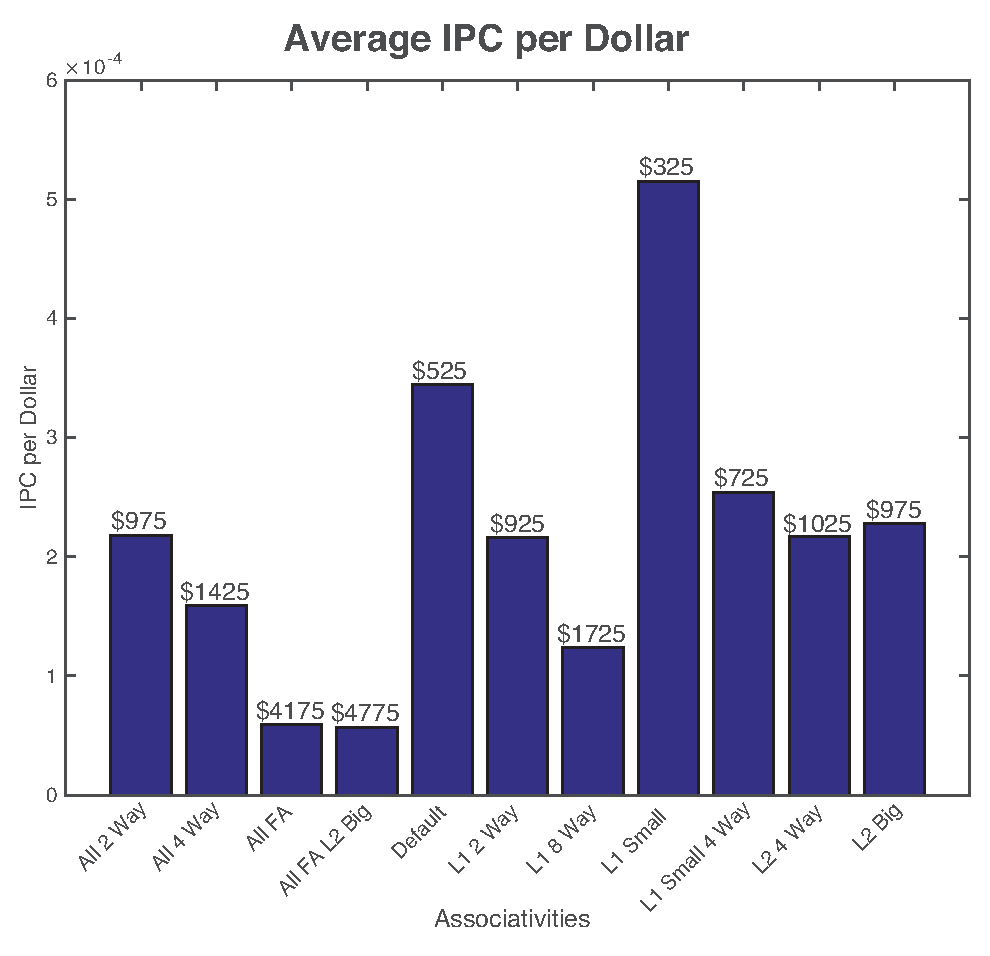
\includegraphics[scale = 0.75]{IPCperDollar.eps}
\caption{Average IPC per Dollar for each configuration\label{fig:IPCperDollar}}
\end{figure}

When choosing a system, Fig.~\ref{fig:IPCperDollar} displays the best performing system for the price. It is however also useful to identify what configuration gives the maximum increase in performance from the cheapest configuration per dollar. Fig.~\ref{fig:deltaIPCperDollar} exhibits these results. L1 small is the cheapest configuration, and from the figure it is apparent that L2 big gives the maximum performance increase per dollar. Interestingly, the FA cases are yield the smallest performance increase per dollar due to their high cost.

\begin{figure}[H]
\centering
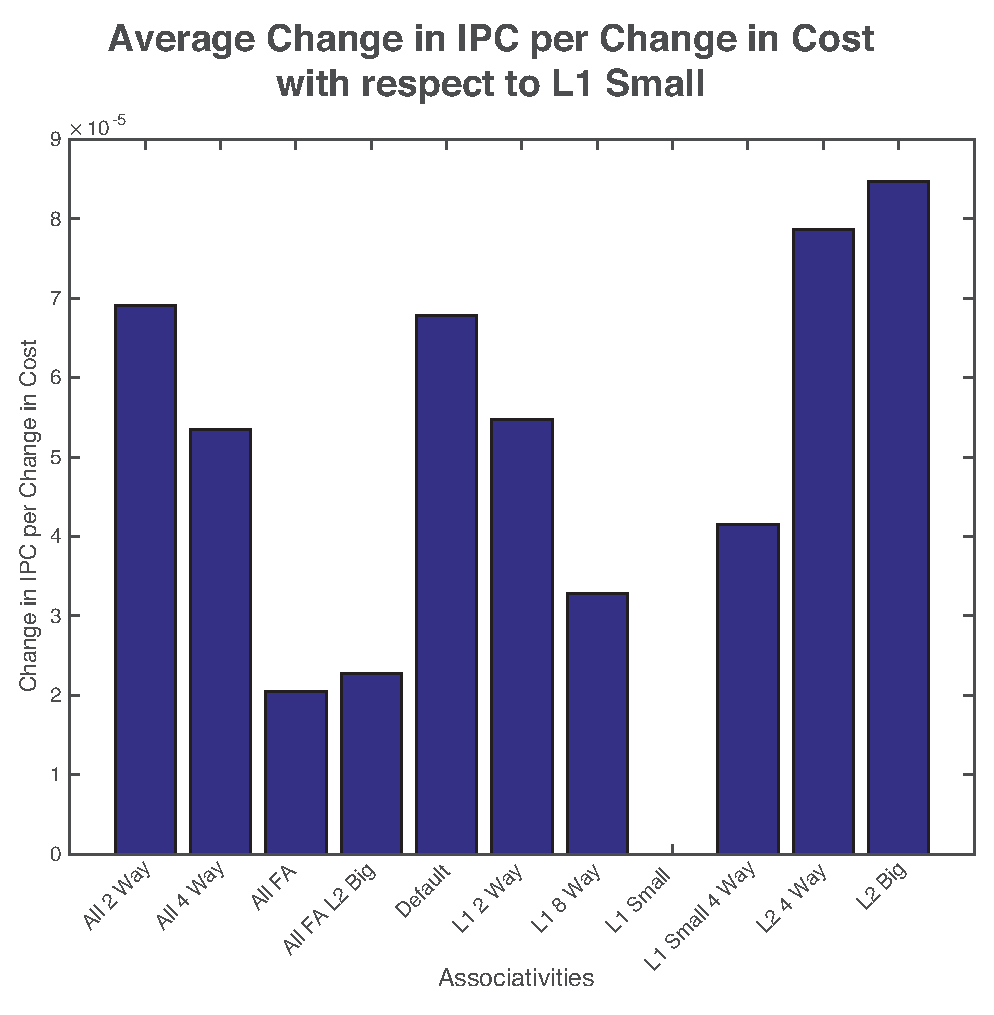
\includegraphics[scale = 0.75]{deltaIPCperdeltaCost.eps}
\caption{Change in average IPC per change in cost for each configuration\label{fig:deltaIPCperDollar}}
\end{figure}

 These results are useful only to selecting a general purpose system.  Clearly, configurations such as libquantum and onmetpp vary considerably in their utilization of the cache structure. Due to the fact that libquantum does not vary in performance over the configurations, it is unnecessary to purchase any cache configuration other than the cheapest case, L1 small. The trace onmetpp has a high variance, and its respective IPC per dollar as well as change in IPC per dollar should be considered for each configuration. The resulting figures can be seen below in Fig.~\ref{fig:omnetppIPCperDollar} and Fig.~\ref{fig:deltaomnetppIPCperDollar}.

\begin{figure}[H]
\centering
\begin{subfigure}[b]{0.49\textwidth}
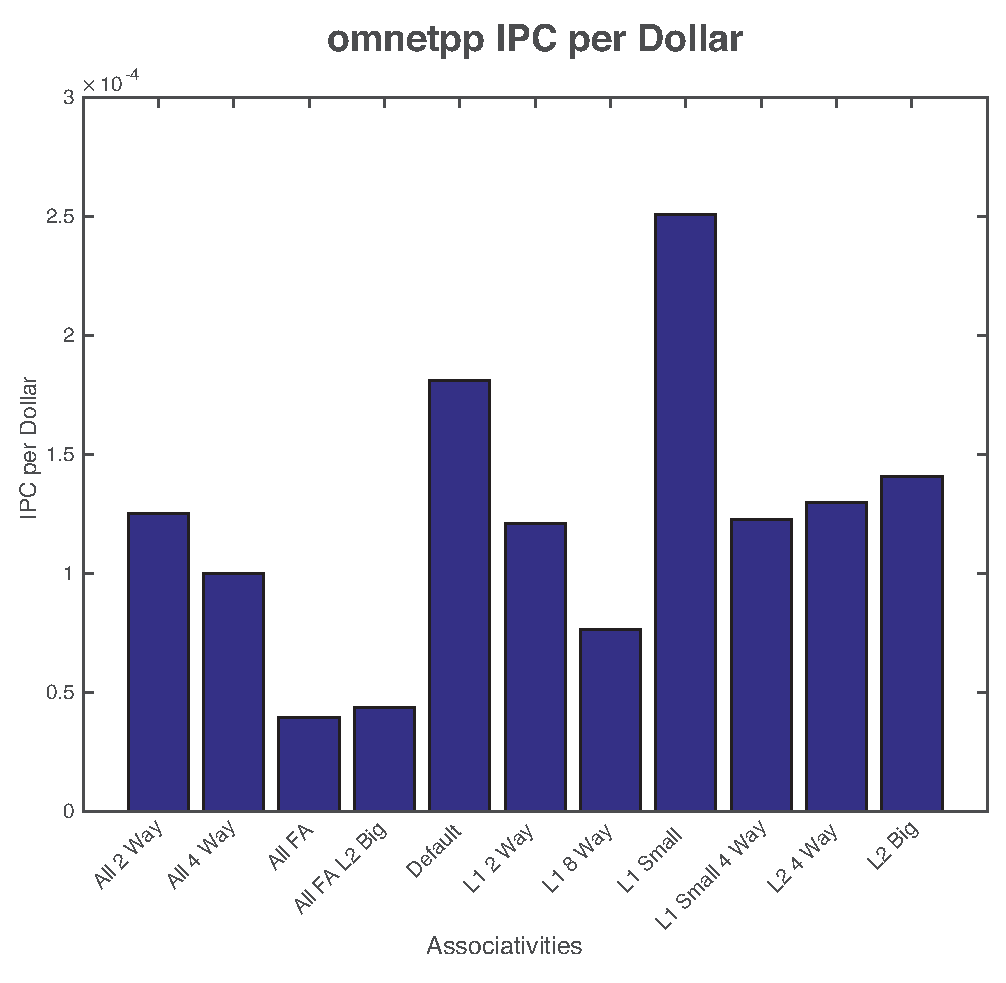
\includegraphics[scale = 0.475]{omnetpp_IPCperDollar.eps}
\caption{IPC per Dollar\label{fig:omnetppIPCperDollar}}
\end{subfigure}
\begin{subfigure}[b]{0.49\textwidth}
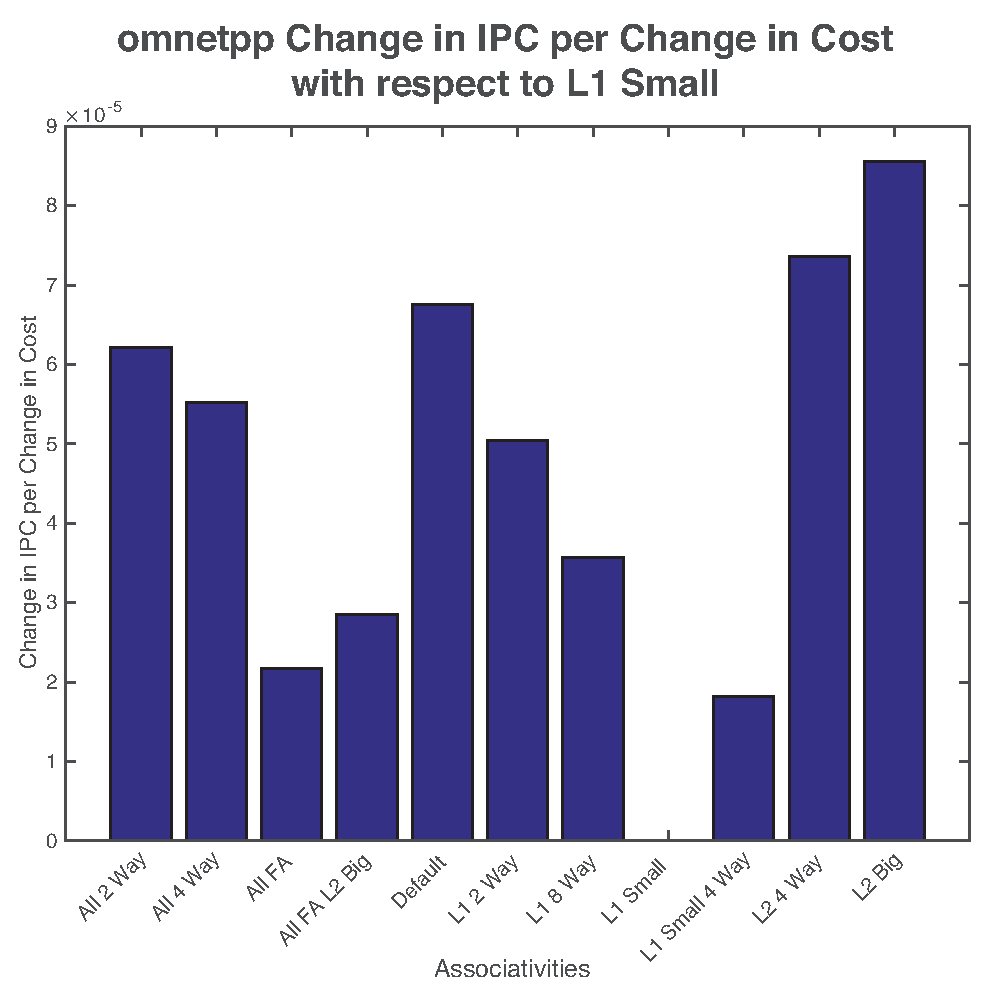
\includegraphics[scale = 0.475]{omnetpp_deltaIPCperdeltaDollar.eps}
\caption{Change in IPC per change in cost\label{fig:deltaomnetppIPCperDollar}}
\end{subfigure}
\caption{omnetpp IPC}\label{fig:omnetpp}
\end{figure}

From the figures above, it is evident that onmetpp follows a similar trend as the averaged case.  

 The chunksize of main memory is an important consideration when evaluating what configuration has the best performance given its cost. The chunksize is the width of the bus interface to memory. Access time to main memory is extremely slow, and so it is beneficial to performance to read as many bytes as possible when memory is accessed. The trade-off is cost, and so it is useful to observe the performance increase versus cost of various configurations of memory chunksize. The default cache configuration for chucksizes of 8, 16, 32, and 64 bytes are compared to their respective costs in Fig.~\ref{fig:chunksizes} below.
 
\begin{figure}[H]
\centering
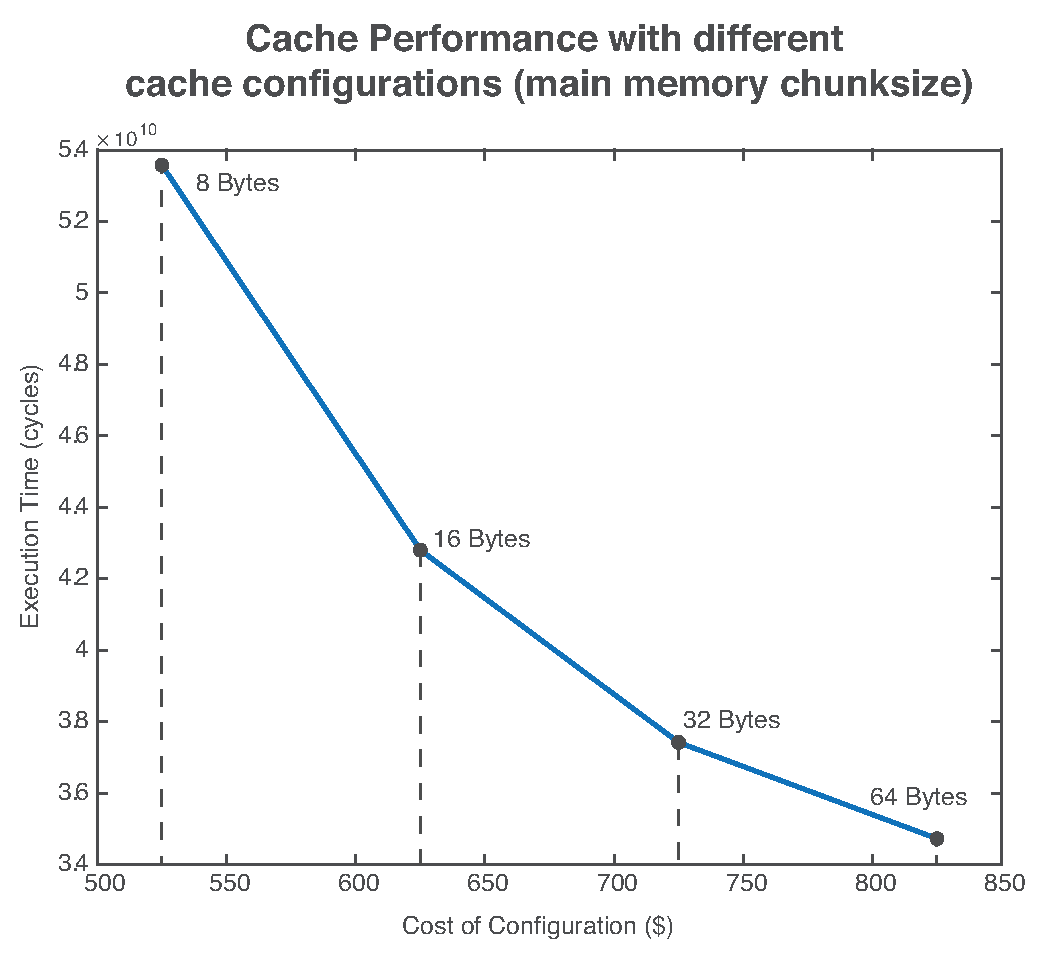
\includegraphics[scale = 0.75]{chunksizeVsCost.eps}
\caption{\label{fig:chunksizes}}
\end{figure}

The largest performance increase occurs between 8 and 16 bytes. As chunksize is further increased, the change in performance begins to decrease. Extrapolating from the graph, it is unlikely that a chunksize greater than 64 bytes would yield a significantly greater performance increase. The performance increase from 8 to 16 bytes is approximately double that of the performance increase from 16 to 32 bytes for the same change in cost.

\end{document}









